\subsection{Szintaktika}

%5
\begin{frame}[fragile]
  \begin{columns}[c]
    \column{0.5\textwidth}
      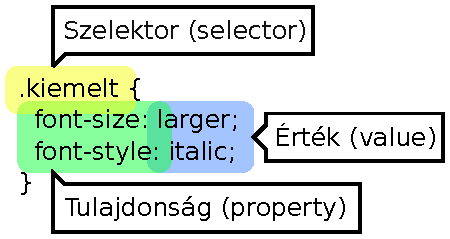
\includegraphics[scale=0.75]{szintakszis.pdf}\\
      \begin{block}{Deklaráció sablonja}
      \vspace{-0.5cm}
\begin{verbatim}
szelektor {
  tulajdonság1: érték(ek);
  tulajdonság2: érték(ek);
  ...
  tulajdonságN: érték(ek);
}
\end{verbatim}
      \vspace{-0.4cm}
      \end{block}
    \column{0.5\textwidth}
      \begin{description}[m]
        \item[Szelektor] \hfill \\ Mit akarunk formázni?
        \item[Tulajdonság] \hfill \\ Milyen tulajdonságán változtassunk?
        \item[Érték] \hfill \\ Milyen legyen az új állapot?
      \end{description}
  \end{columns}
  
\end{frame}

%6
\begin{frame}
  Megjegyzések a CSS-ben:
  \begin{itemize}
    \item \texttt{/* megjegyzes */}
    \item végleges kódból célszerű elhagyni
    \item Lehet több soros is
  \end{itemize} 
  \hiv{\href{https://jigsaw.w3.org/css-validator/}{CSS ellenőrző}}\\
  \hiv{\href{https://jsfiddle.net/}{JSFiddle - Code Playground}}\\
  Böngésző Webfejlesztő menüje (F12), stílusszerkesztő
\end{frame}
